The initial QoE-predictive scheduler uses point forecasts of each path. The calibrated upper bound $\hat{q}_{0.975}+c$ of the final model is a per-path, per-step RTT bound that holds about 95\% of the time on unseen sessions. Because it depends on the input, it is tight when a path is stable and loose only when the path is about to burst. A constant-width bound is equally wide at all times. This section measures what that difference is worth (script \texttt{fr\_scheduler.py}).

\paragraph{Emulation.} We emulate deadline-aware packet duplication on the test sessions of the four satellite links, with the satellite path as primary and the 5G path of the same direction as backup. At time $t$ the scheduler plans the packets it will send at $t+h$, $h\in\{0.2,\dots,3\}$\,s. A packet on the primary misses its deadline $D$ if the measured RTT at $t+h$ exceeds $D$, set to the 90th percentile of the calibration-session RTT (\SchedDSLDL\,ms on Starlink DL). The scheduler duplicates a packet on the backup when its forecast bound exceeds $D$. We count the share of duplicated packets, which costs backup capacity, and the share of late packets that were not duplicated (misses).

\begin{figure}[htbp]
  \centering
  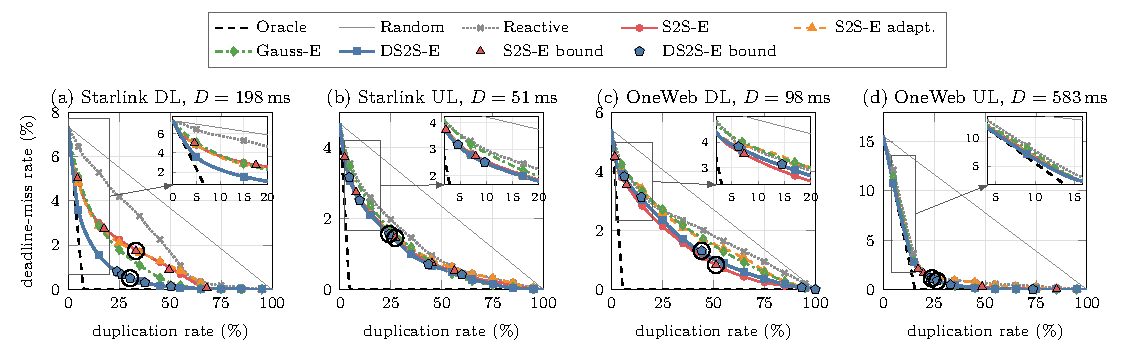
\includegraphics[width=\linewidth]{figs_pdf/fr_scheduler.pdf}
  \caption{Deadline-aware duplication on the test sessions: share of late, non-duplicated packets against the share of duplicated packets, pooled over 0.2--3\,s. Curves sweep the knob of each policy. Markers: one-sided bounds calibrated at 0.80 to 0.99, circled at 0.95. Insets: low duplication. S2S-E adapt.\ scales its margin by the input volatility.}
  \label{fig:sched}
\end{figure}

\paragraph{Deployable comparison.} A deployed scheduler must set its knob in advance. For S2S-E we use the one-sided 95\% conformal upper bound. For DS2S-E we set the knob on the calibration sessions so that its miss rate there equals that of the S2S-E bound. On Starlink DL, the S2S-E bound duplicates \SchedSSdupSLDL\% of the packets and misses \SchedSSmissSLDL\%. DS2S-E duplicates \SchedDSdupSLDL\% and misses \SchedDSmissSLDL\%, which is \SchedSaveSLDL\% less duplication (95\% CI \SchedSaveSLDLlo{} to \SchedSaveSLDLhi\%) with no more misses. On Starlink UL and OneWeb UL the two schedulers tie (duplication change \SchedSaveSLUL\% and \SchedSaveOWUL\%). On OneWeb DL, DS2S-E needs \SchedDSdupCurveOWDL\% duplication to reach the miss rate of the S2S-E bound, which duplicates \SchedSSdupOWDL\%. Every forecaster with the anchored decoder loses there, including the point forecaster S2S-AE-E, so the loss comes from the decoder and not from the distributional output. The same decoder ranks the rare OneWeb DL spikes worse (AUROC \AUCFROWDL{} against \AUCPrevOWDL{} for the initial model), while on Starlink DL it is the best spike warning (\AUCFRSLDL{} against \AUCPrevSLDL).

\paragraph{Where the gain comes from.} At the miss rate of the S2S-E bound on Starlink DL, S2S-AE-E needs \SchedFFdupSLDL\% duplication, DS2S-E \SchedDSdupCurveSLDL\%, and S2S-E \SchedSSdupCurveSLDL\%. About half of the gain comes from the new inputs and decoder and half from the predictive distribution. \GaussSchedSentence{} The saving is largest for deadlines between the 90th and 97.5th percentile and at short lead times. It shrinks for the 99th percentile, which lies beyond the 97.5\% quantile that DS2S-E describes.

\paragraph{Same mean, different risk.} Fig.~\ref{fig:risk} groups the test windows by the S2S-E mean forecast and, within each group, by the spread that DS2S-E predicts. At the same mean forecast of \RiskMeanLo{} to \RiskMeanHi\,ms on Starlink DL, \RiskLowPct\% of the packets are late when DS2S-E predicts a narrow spread and \RiskHighPct\% when it predicts a wide one. A scheduler that sees only the mean must treat these windows alike.

\begin{figure}[htbp]
  \centering
  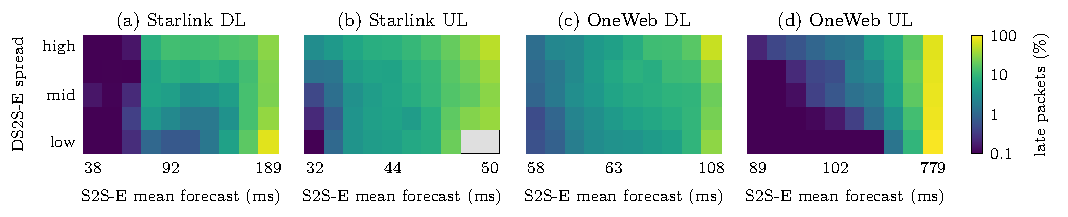
\includegraphics[width=\linewidth]{figs_pdf/fr_scheduler_risk.pdf}
  \caption{Same mean, different risk. Share of late packets (log color scale) when the test windows are grouped by the S2S-E mean forecast (deciles, x) and, within each decile, by the predicted DS2S-E spread $\hat{q}_{0.975}-\hat{q}_{0.5}$ (quintiles, y).}
  \label{fig:risk}
\end{figure}

\paragraph{Caveats.} Only the bound-against-bound comparison is deployable. The curves sweep each knob on the test windows, like an ROC curve. On the test sessions the one-sided 95\% bounds covered \BoundCovLo{} to \BoundCovHi{} of the RTT values. The satellite and 5G sessions were not recorded at the same time, so the emulation assumes independent paths. If they are, the 5G UL backup itself exceeds the Starlink UL deadline in \BackupQULSL\% of its samples, which raises the DS2S-E miss rate on Starlink UL from \BackupDSmissSLUL\% to \BackupDSmissCorrSLUL\%.
